% !TEX root = ../thesis_main.tex


%%%% --- * --- %%%%
\clearpage	

\chapter{The Experimental Signature}
\label{analysis_chapter}

\section{TBD}
\note[color=jb]{JB:  You need to at some point say that the supersum is the beta energy spectrum.  There are experiments trying to do this method better, but they are very difficult.  UCNA published a combined energy spectrum and Abeta[Ebeta] analysis on the neutron in March 2020~\cite{NeutronbFierz_March2020}.}
\note{I can't help but also notice the follow-up article from September 2020~\cite{NeutronbFierz_September2020}.  Ugh. }
I really need an excuse to include more pictures of data.  Also, more pictures of simulations.

\missingfigure{Show individual beta energy spectra.  ...with a variety of different cuts, perhaps?}

\missingfigure{Show simulated spectra separated by scattering category.}

\missingfigure{Show SimpleMC spectra, show the supersum, show the superratio, show the superratio asymmetry.  Maybe do some simple fits to show how much better the superratio asymmetry is than \emph{not} the superratio asymmetry.  }


\section{The Superratio and Asymmetry}
%\\*
The data can be combined into a superratio asymmetry.  This has the benefit of causing many systematics to cancel themselves out at leading order.  It also will increase the fractional size of the effects we're looking for.  This can be shown by using math.  

\section{Signature of a Fierz Term in This Experiment}
%\\*
Not all systematics effects are eliminated.  We'll want to be careful to propagate through any effects that are relevant.  Using the superratio asymmetry as our physical observable makes this process a bit messier for the things that don't cancel out, but it's all just math.  

\section{Comparative Merits of the Superratio and Supersum for Measurement}
%\\*
Some other groups have performed similar measurements using the supersum as the physical observable.  There are pros and cons to both methods.  I can show, using a back-of-the-envelope calculation, that for this particular dataset, the superratio asymmetry method produces a better result.  

\begin{figure}[h!!t]
	\centering
	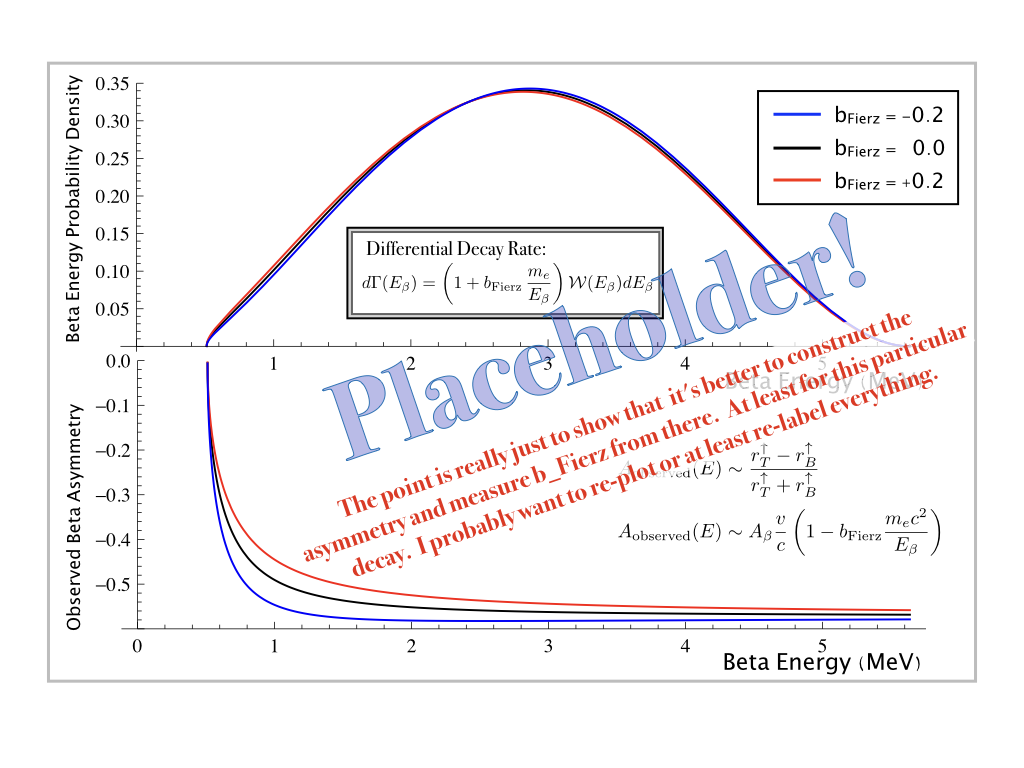
\includegraphics[width=.999\linewidth]
	{Figures/SuperSumSuperRatio_prelim}
	\caption{Here's why it's better to extract $\bFierz$ from an asymmetry, in this case.}	
	\label{fig:supersumsuperratio}
\end{figure}

